\documentclass{article}

\usepackage{fullpage}
\usepackage{amsmath}
\usepackage{bm}
\usepackage{tabu}
\usepackage{graphicx}

\begin{document}

\title{Effects of Different Average Types for Spatial Discretization of Stochastic Flux for Small-Number-of-Particles-in-a-Cell Case\footnote{The arithmetic-mean average type currently implemented in the codes is different from the one discussed in this report. Please read the subsequent report (\texttt{repo2} in the same directory). Note that based on the results present in these two reports the current version of \texttt{avg\_type=1} has been implemented.}~\footnote{For the actual run script, inputs file, and post-processing scripts, see \texttt{exec/reactDiff/test/misc/Schlogl\_hist\_1d}.}}

\date{}

\maketitle

\section{Aim}

Various spatial average types for the stochastic flux generation, which were implemented in the codes, have been tested for the case where the number of particles in each cell is very small.
Their resulting behaviors on the number density distribution and the structure factor have been investigated by comparing numerical results with theoretical predictions obtained from the large-number-of-particles-in-a-cell case.
To minimize the effects of a temporal integrator, a very small time step was used.
One-dimensional diffusion-only and reaction-diffusion cases were considered. 

In addition, numerical results were also obtained from the multinomial diffusion scheme (plus the SSA scheme for reaction) and it has been confirmed that the theoretical predictions hold even in the small-number-of-particles-in-a-cell case and the latter scheme can provide the right answer in the small time step limit.

\section{Average Types for Spatial Discretization of Stochastic Flux}

For the one-dimensional diffusion-only case
\begin{equation}
\frac{\partial}{\partial t}n(x,t)=\chi\frac{\partial^2}{\partial x^2}n(x,t)+\frac{\partial}{\partial x}\left[\sqrt{2\chi n(x,t)} \bm{\mathcal{W}}(x,t)\right],
\end{equation}
the spatial discretization used in the code is as follows:
\begin{equation}
\frac{d}{dt}n_j(t) = \chi \frac{n_{j+1}(t)+n_{j-1}(t)-2n_j(t)}{\Delta x^2}
+\frac{1}{\Delta x^{3/2}}\left[
\sqrt{2\chi\tilde{n}_{j+\frac12}(t)} W_{j+\frac12}(t)
-\sqrt{2\chi\tilde{n}_{j-\frac12}(t)} W_{j-\frac12}(t)
\right].
\end{equation}
For the compuation of $\sqrt{2\chi \tilde{n}}$ in the stochastic flux term, the face value $\tilde{n}$ between two cells needs to be approximated by their center values $n_1$ and $n_2$.
In the codes, the following three average types have been implemented: arithmetic mean, geometric mean, and harmonic mean.

If negative densities occur, however, there may be some issues; the face value may not be well-defined or may be negative.
In this case, additional treatment is needed.
In the code, the following rules are applied:
\begin{center}
{\tabulinesep=1.2mm
\begin{tabu}{|c|c|c|}
\hline
Average type & if $n_1>$0 and $n_2>0$ & if $n_1<0$ or $n_2<0$ \\
\hline
Arithmetic (\texttt{avg\_type=1}) & $\frac{1}{2}(n_1+n_2)$ & $\frac{1}{2}\left[\mathrm{max}(n_1,0)+\mathrm{max}(n_2,0)\right]$ \\
\hline
Geometric (\texttt{avg\_type=2}) & $\sqrt{n_1 n_2}$ & 0 \\
\hline
Harmonic (\texttt{avg\_type=3}) & $\frac{2}{n_1^{-1}+n_2^{-1}}$ & 0 \\
\hline
Arithmetic (\texttt{avg\_type=4}) & $\frac{1}{2}(n_1+n_2)$ & 0 \\
\hline
\end{tabu}
}
\end{center}
Note that a new arithmetic average type (\texttt{avg\_type=4}) has been added.
The difference between two arithmetic average types is that the new one becomes zero when $n_1$ or $n_2$ becomes negative (as in \texttt{avg\_type=2} or \texttt{3}), whereas the old one becomes zero only when both $n_1$ and $n_2$ become negative.

If each cell has a large number of particles, it is expected that there are not such issues and there are no significant differences among different average types.
This is because negative densities may not occur since the stochastic flux is small.
Also, face values obtained from different average types are rather similar since the two center values are similar due to small fluctuation in the number density.

\section{Numerical Calculations}

\subsection{Systems}

The diffusion-only and reaction-diffusion cases were calculated.
Since the former corresponds to the case obtained by simply turning off the reaction part in the latter case, numerical details are explained for the reaction-diffusion system.

The one-dimensional Schlogl model satisfying detailed balance was calculated on a grid having 64 cells with $\Delta x=1$.
The diffusion coefficient was given as $\chi=1$ and reaction constants were given as $k_1=k_2=k_3=k_4=0.1$.
In this case, the equilibrium number density is $n_\mathrm{eq}=1$.
The cross section was chosen as $\Delta A=5$ so that the average number of particles in a cell is $N=n_\mathrm{eq}\Delta V=5$.

For a temporal integrator, the unsplit explicit midpoint scheme with \texttt{midpoint\_stoch\_flux\_type=2} was employed with time step $\Delta t=0.01$.
Fluctuations of the reaction part was described by Poisson random numbers (i.e., the tau-leaping method) rather than by Gaussian random numbers (i.e., the chemical Langevin equation). 
Since the time step is small, the effects of the specific temporal integrator (and its specific option \texttt{midpoint\_stoch\_flux\_type}) is expected to be negligible.
By comparing results with those obtained from the unsplit implicit midpoint scheme and/or different option values, this has been confirmed. 

For comparison, the first-order splitting scheme combining the multinomial diffusion and the SSA scheme for reaction was also calculated.

The initial distribution of the number density $n$ was generated by using the following options: for the diffusion-only case, \texttt{initial\_variance=-1} (with fluctuation, but its total sum is zero) and \texttt{integer\_populations=F} for the explicit midpoint scheme, and \texttt{initial\_variance=0} (without fluctuation) and \texttt{integer\_populuations=T} for the multinomial diffusion; for the reaction-diffusion case, \texttt{initial\_variance=1} (with fluctuation and no constraint on its total sum) and \texttt{integer\_populations=F} for the explicit midpoint scheme, and \texttt{initial\_variance=1} and \texttt{integer\_populuations=T} for the multinomial diffusion + SSA reaction.

\subsection{Physical Quantities}

The following three physical quantities were obtained for analysis:
\begin{itemize}
\item Number density distribution $\rho(n)$,
\item Structure factor $S(k)$,
\item Variance $\mathrm{Var}[n]$.
\end{itemize}

These quantities were obtained from the cell number density data $\{n_j(i\Delta t)\}$ $(j=1,\dots,64)$.
The first $10^5$ steps for equilibration were discarded and then the data at every five steps for the next $10^6$ steps were used.
For the calculation of the histogram, the number of particles $n\Delta V$ was rounded to the nearest integer and then the corresponding number density was used for binning.
From a total of 16 runs with different random seeds, the standard errors were also estimated.   

\subsection{Comparison with theoretical predictions}

\begin{itemize}
\item $\rho(n)$: Since the number of particles in a cell is expected to obey the Poisson distribution with mean $N=n_\mathrm{eq}\Delta V$, the corresponding distribution for the number density was calculated and compared.
\item $S(k)$: Owing to the equilibrium state, $S(k)$ is expected to be flat except at $k=0$ with the value $S(k)=n_\mathrm{eq}=1$.
\item $\mathrm{Var}[n]$: From the Poisson distribution for the number of particles, it is expected that $\mathrm{Var}[n]=n_\mathrm{eq}/\Delta V=0.2$.
\end{itemize}

\noindent The following relation between $S(k)$ and $\mathrm{Var}[n]$ may be useful for the interpretation of numerical results: 
\begin{equation}
\label{sumSknonzero}
\frac{1}{V}\sum_{k\ne0}S(k)\approx \mathrm{Var}[n].
\end{equation}
Roughly speaking, an overall change in $S(k)$ should be reflected on $\mathrm{Var}[n]$ and vice versa.
For the derivation, see the Appendix.

\section{Results}

\subsection{Diffusion-Only Case}

\begin{figure}[ht!]
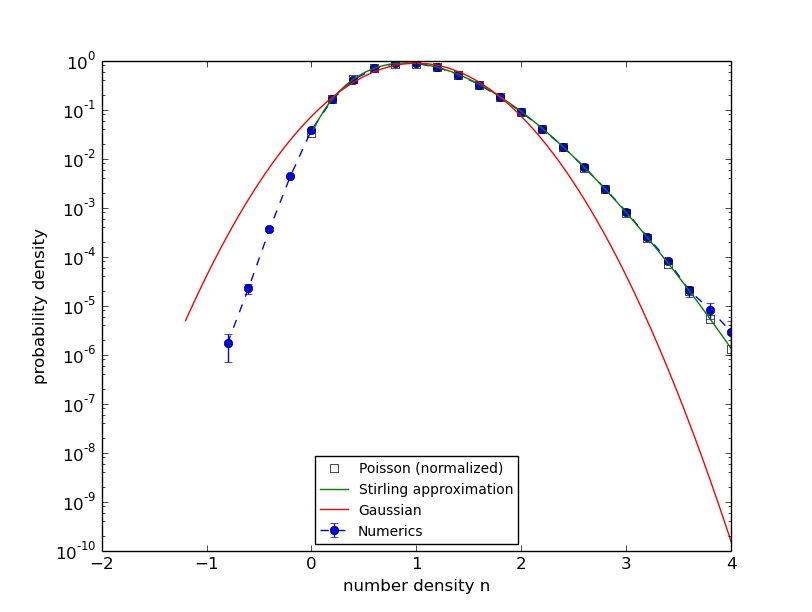
\includegraphics[width=0.5\linewidth]{fig1/diff_hist_avg1.jpg}
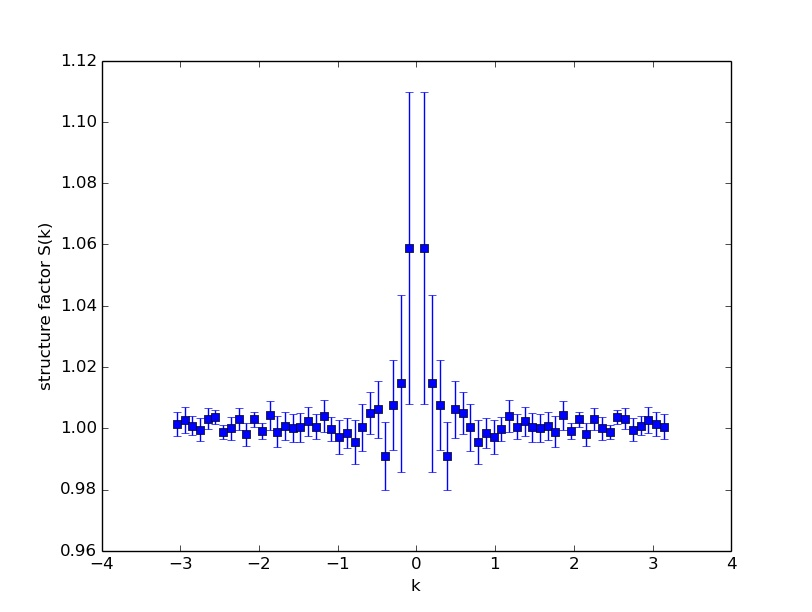
\includegraphics[width=0.5\linewidth]{fig1/diff_Sk_avg1.jpg}
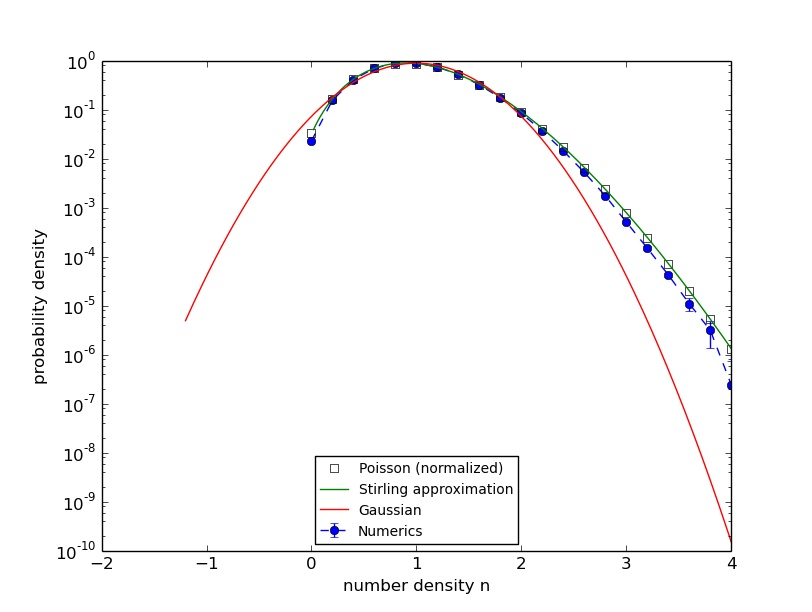
\includegraphics[width=0.5\linewidth]{fig1/diff_hist_avg2.jpg}
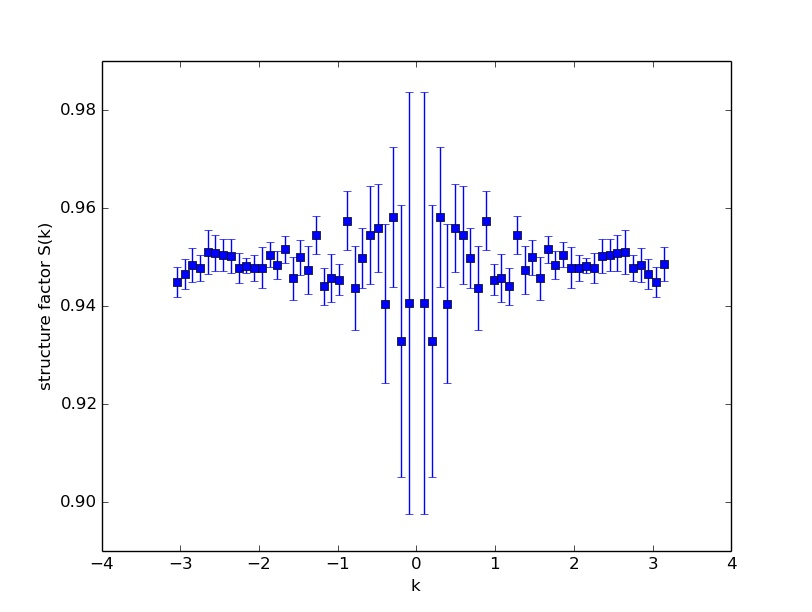
\includegraphics[width=0.5\linewidth]{fig1/diff_Sk_avg2.jpg}
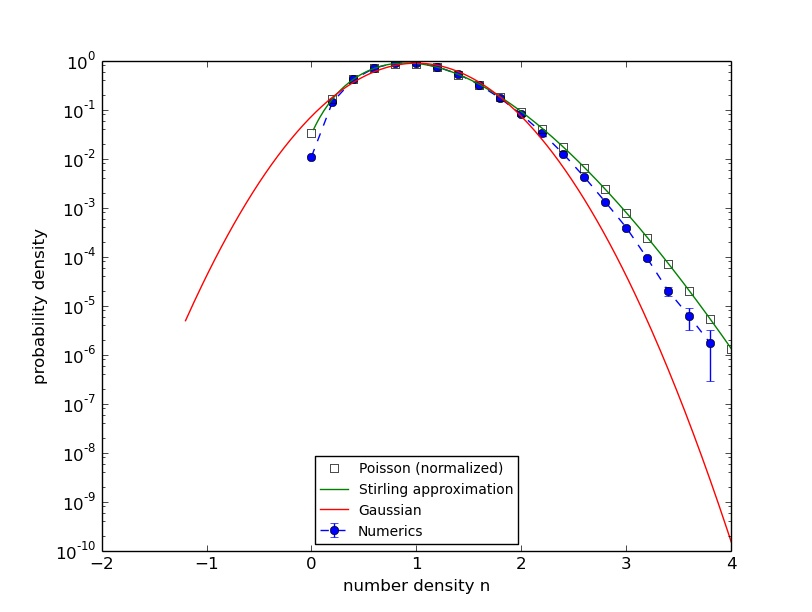
\includegraphics[width=0.5\linewidth]{fig1/diff_hist_avg3.jpg}
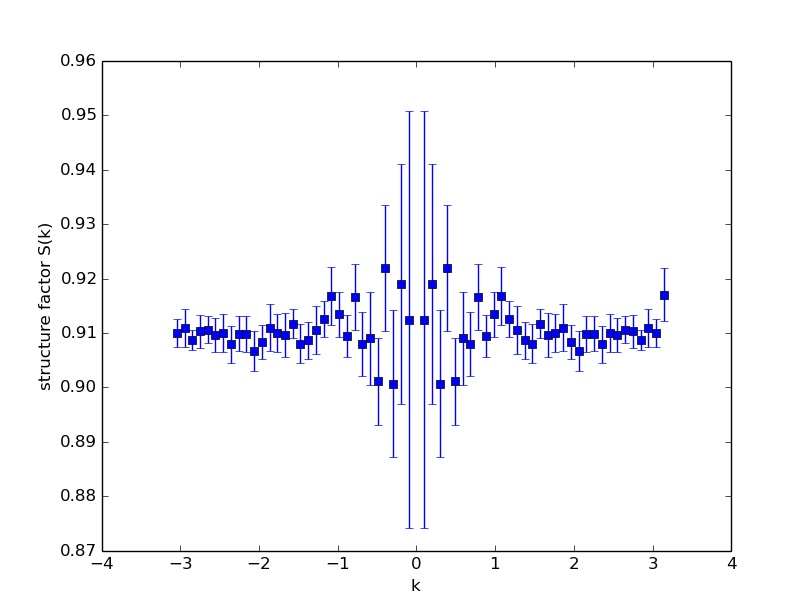
\includegraphics[width=0.5\linewidth]{fig1/diff_Sk_avg3.jpg}
\caption{\label{fig_diff_123}[Diffusion-only case] Results of $\rho(n)$ (left column) and $S(k)$ (right column) for \texttt{avg\_type=1} (old arithmetic mean, top row), \texttt{avg\_type=2} (geometric mean, middle row), and \texttt{avg\_type=3} (harmonic mean, bottom row).
}
\end{figure}

\begin{figure}[ht!]
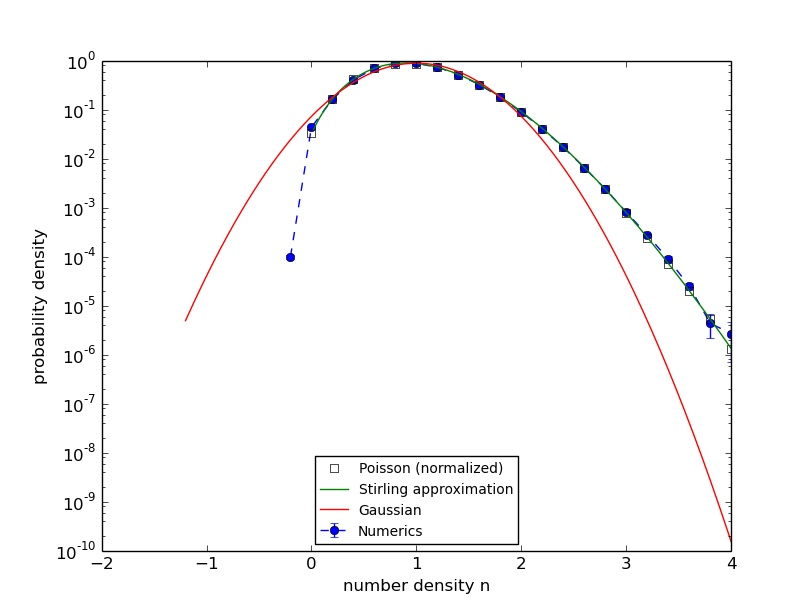
\includegraphics[width=0.5\linewidth]{fig1/diff_hist_avg4.jpg}
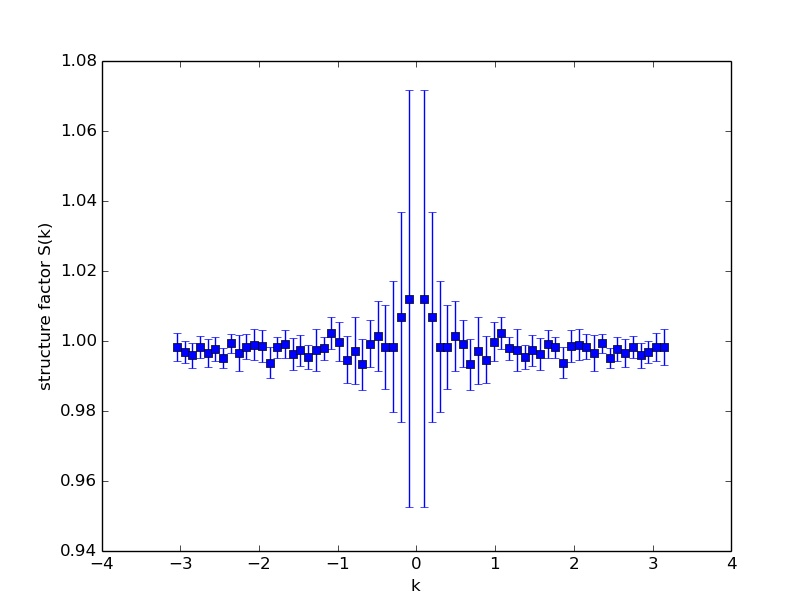
\includegraphics[width=0.5\linewidth]{fig1/diff_Sk_avg4.jpg}
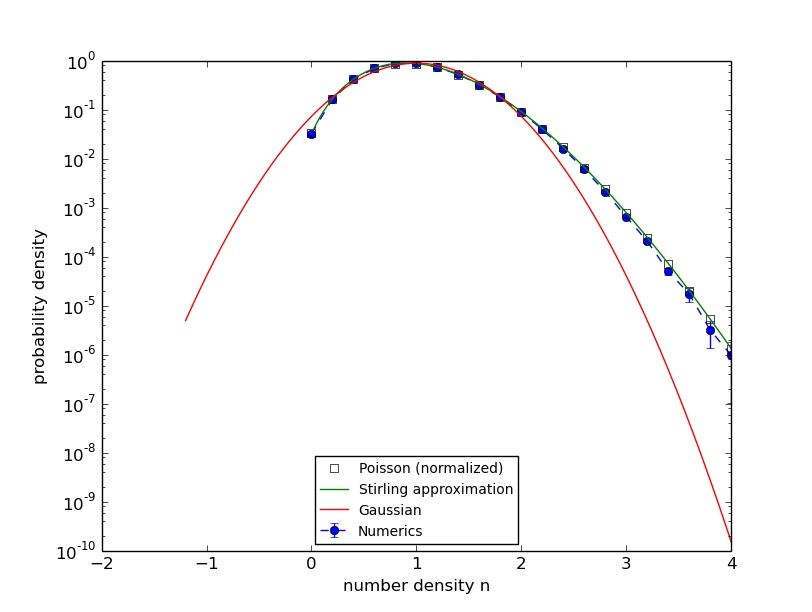
\includegraphics[width=0.5\linewidth]{fig1/diff_hist_mn.jpg}
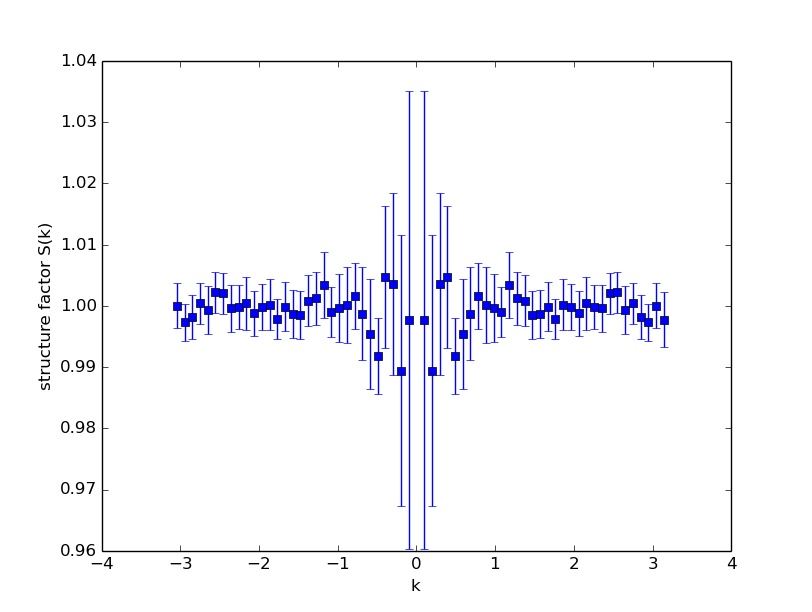
\includegraphics[width=0.5\linewidth]{fig1/diff_Sk_mn.jpg}
\caption{\label{fig_diff_45}[Diffusion-only case] Results of $\rho(n)$ (left column) and $S(k)$ (right column) for \texttt{avg\_type=4} (new arithmetic mean, top row) and the multinomial diffusion (bottom row).
}
\end{figure}

Figures~\ref{fig_diff_123} and \ref{fig_diff_45} show $\rho(n)$ and $S(k)$ for various \texttt{avg\_type} and the multinomial diffusion.
In the multinomial diffusion method, both physical quantities agree very well with the theoretical predictions. 
For the old arithmetic mean (\texttt{avg\_type=1}), negative densities are observed although all the other behaviors seem fine.
For the new arithmetic mean (\texttt{avg\_type=4}), negative densities are hardly observed and all the other behaviors also seem fine. 
For the geometric mean (\texttt{avg\_type=2}), although negative densities are not observed, deviations of $\rho(n)$ from the Poisson distribution are observed and the flat value of $S(k)$ is smaller than $n_\mathrm{eq}$. 
For the harmonic mean (\texttt{avg\_type=1}), similar behaviors to the geometric mean case are observed but the deviations are even larger.

The variance of $n$ is as follows:
\begin{center}
{\tabulinesep=1.2mm
\begin{tabu}{|c|c|}
\hline
Average type & $\mathrm{Var}[n]$ (standard error) \\
\hline
Arithmetic (\texttt{avg\_type=1}) & 0.1975 (0.0002) \\
\hline
Geometric (\texttt{avg\_type=2}) & 0.1867 (0.0002) \\
\hline
Harmonic (\texttt{avg\_type=3}) & 0.1792 (0.0002) \\
\hline
Arithmetic (\texttt{avg\_type=4}) & 0.1965 (0.0002) \\
\hline
Multinomial diffusion & 0.1967 (0.0002) \\
\hline
\end{tabu}
}
\end{center}
As expected from Eq.~\eqref{sumSknonzero}, for the geometric and harmonic means, the deviation of $\mathrm{Var}[n]$ from the true value is significant. 

\subsection{Reaction-Diffusion Case}

\begin{figure}[ht!]
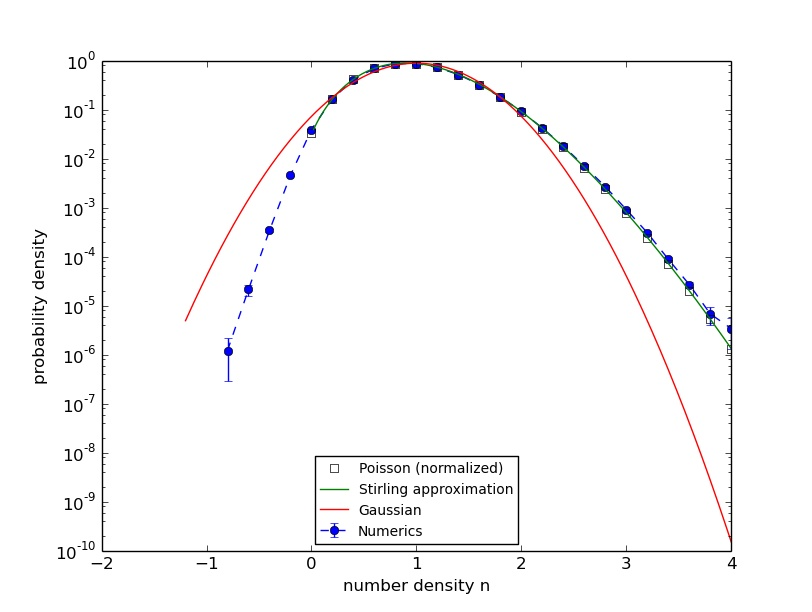
\includegraphics[width=0.5\linewidth]{fig1/react_hist_avg1.jpg}
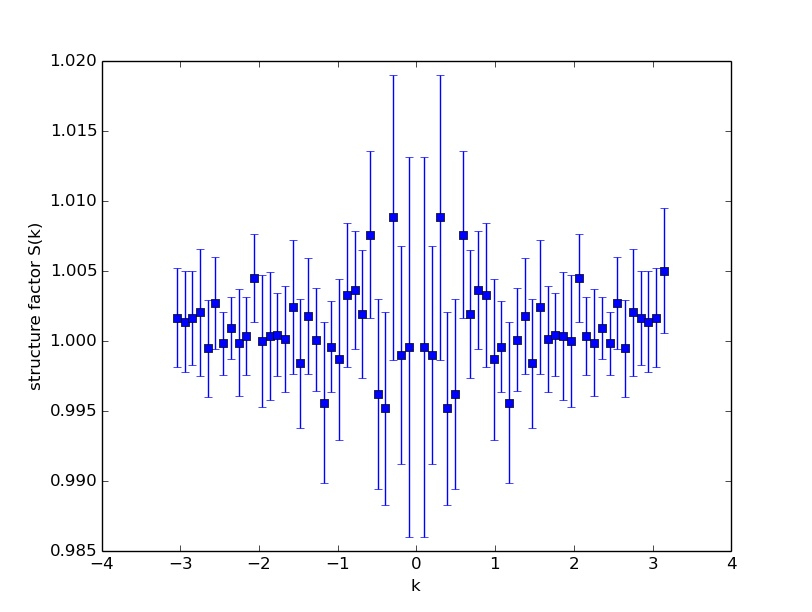
\includegraphics[width=0.5\linewidth]{fig1/react_Sk_avg1.jpg}
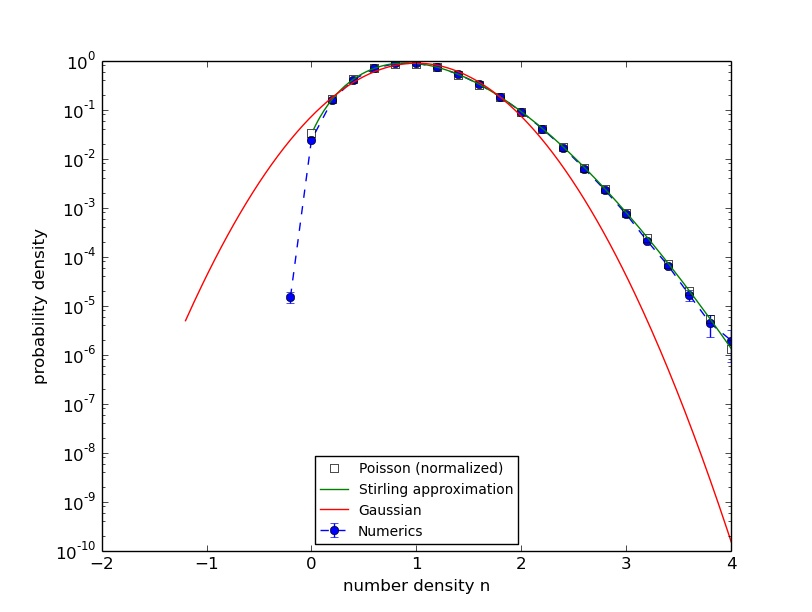
\includegraphics[width=0.5\linewidth]{fig1/react_hist_avg2.jpg}
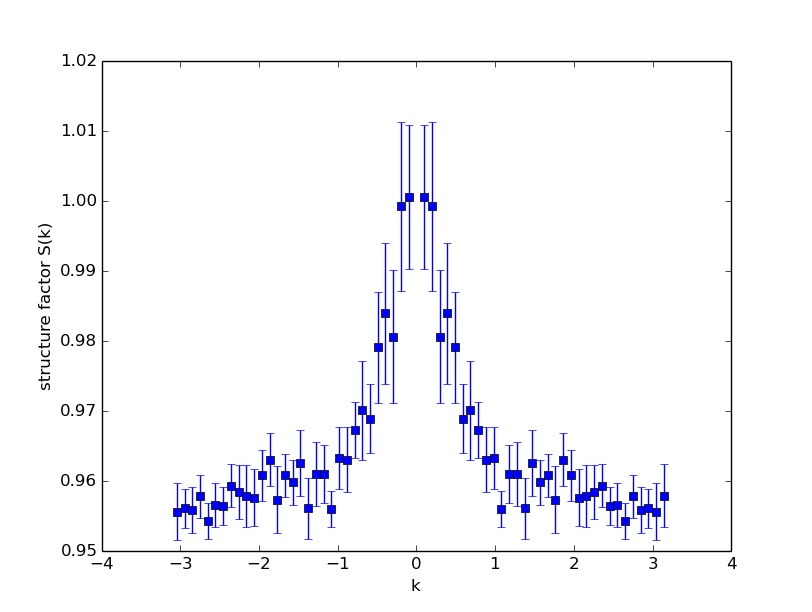
\includegraphics[width=0.5\linewidth]{fig1/react_Sk_avg2.jpg}
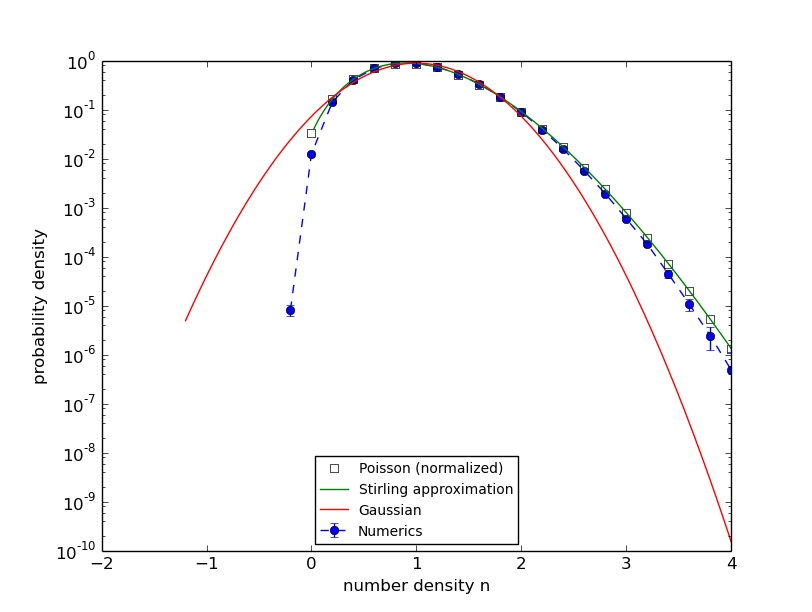
\includegraphics[width=0.5\linewidth]{fig1/react_hist_avg3.jpg}
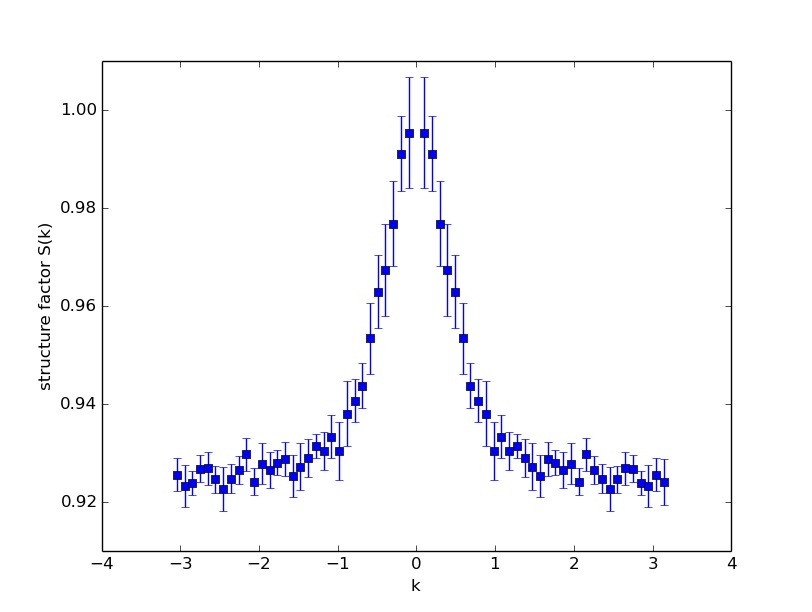
\includegraphics[width=0.5\linewidth]{fig1/react_Sk_avg3.jpg}
\caption{\label{fig_react_123}[Reaction-diffusion case] Results of $\rho(n)$ (left column) and $S(k)$ (right column) for \texttt{avg\_type=1} (old arithmetic mean, top row), \texttt{avg\_type=2} (geometric mean, middle row), and \texttt{avg\_type=3} (harmonic mean, bottom row).
}
\end{figure}

\begin{figure}[ht!]
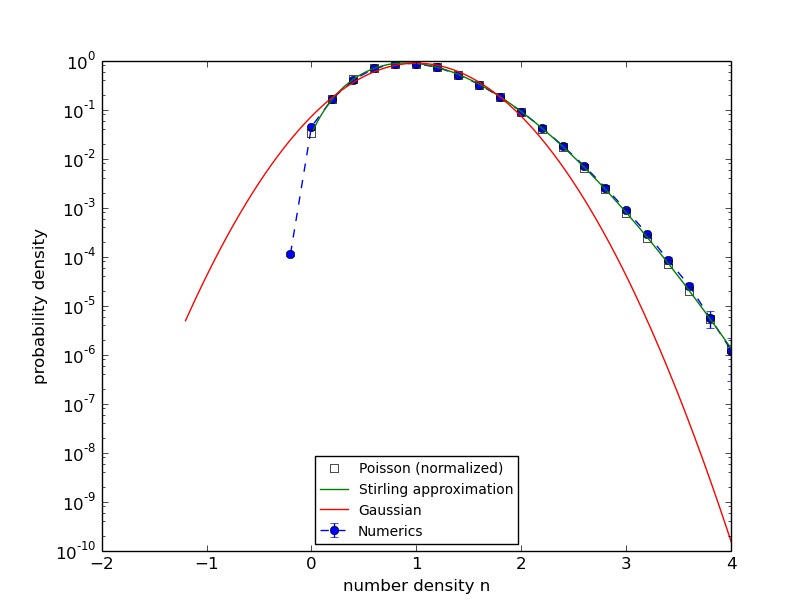
\includegraphics[width=0.5\linewidth]{fig1/react_hist_avg4.jpg}
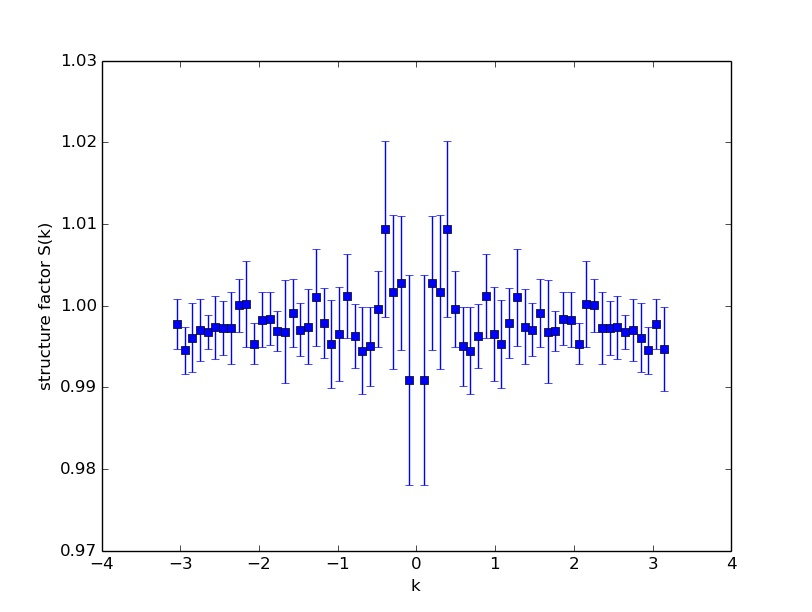
\includegraphics[width=0.5\linewidth]{fig1/react_Sk_avg4.jpg}
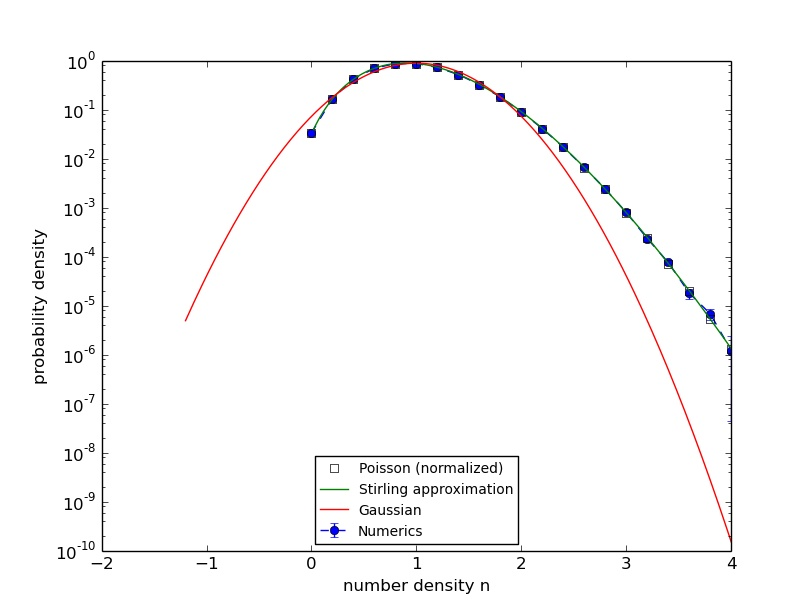
\includegraphics[width=0.5\linewidth]{fig1/react_hist_mn.jpg}
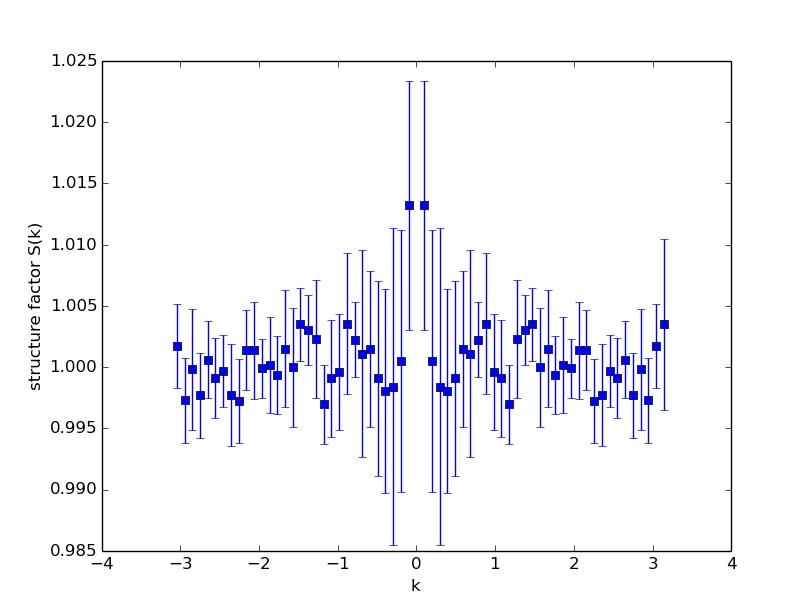
\includegraphics[width=0.5\linewidth]{fig1/react_Sk_mn.jpg}
\caption{\label{fig_react_45}[Reaction-diffusion case] Results of $\rho(n)$ (left column) and $S(k)$ (right column) for \texttt{avg\_type=4} (new arithmetic mean, top row) and the multinomial diffusion + SSA (bottom row).
}
\end{figure}

Unfavorable behaviors that each average type exhibits are similar to the diffusion-only case.
However, note that although the same flat shape of $S(k)$ is theoretically predicted as in the diffusion-only case, the shape of $S(k)$ obtained for the geometric and harmonic means are not flat. 
The variance of $n$ is as follows:
\begin{center}
{\tabulinesep=1.2mm
\begin{tabu}{|c|c|}
\hline
Average type & $\mathrm{Var}[n]$ (standard error) \\
\hline
Arithmetic (\texttt{avg\_type=1}) & 0.2002 (0.0001) \\
\hline
Geometric (\texttt{avg\_type=2}) & 0.1930 (0.0001) \\
\hline
Harmonic (\texttt{avg\_type=3}) & 0.1876 (0.0001) \\
\hline
Arithmetic (\texttt{avg\_type=4}) & 0.1995 (0.0001) \\
\hline
Multinomial diffusion + SSA & 0.2001 (0.0001) \\
\hline
\end{tabu}
}
\end{center}

\section{Interpretation}

\subsection{Negative densities}

Compared with the other average types, the old arithmetic mean exhibits significant probability of negative densities.
This can be explained as follows.
If one cell has a negative density and the other cell has a positive density, all the other average types do not allow any stochastic flux.
However, the old arithmetic mean average type determines a positive value of the face value and allows stochastic flux.
Hence, there is probability $1/2$ that the negative density becomes even more negative.

However, it is noted that even after the old arithmetic mean is replaced by the new arithmetic mean, the arithmetic mean average type has more chance of negative densities than the geometric and harmonic means. This can be explained by the following well-known inequalities:
\begin{equation}
\label{inequil}
\mbox{(arithmetic mean)}\ge\mbox{(geometric mean)}\ge\mbox{(harmonic mean)}.
\end{equation}
When two cells have positive densities, if two values are very different in magnitude, three means become very different.
Hence, the arithmetic mean average type has larger stochastic flux than the other two and has more chance of negative densities.

\subsection{Smaller variance of $n$}

Smaller variance than the true value is attributed to the following two artificial treatments.
The first one is zeroing of the face value due to negative densities; the more zeroing occurs, the smaller the variance becomes.
The second one is the approximation of the face value by other mean values than the arithmetic mean;
from \eqref{inequil}, if other mean values are used, the variance becomes smaller. 
The effects of the first reason can be assessed by comparing \texttt{avg\_type=1} and \texttt{4}, whereas those of the second reason can be investigated from \texttt{avg\_type=2}, \texttt{3}, and \texttt{4}.

\subsection{Tentative conclusion for the best average type}

Compared with the geometric and harmonic mean average types, both arithmetic average types exhibit much better $S(k)$, $\rho(n)$, and $\mathrm{Var}[n]$.
From a criterion of smaller chance of negative densities, the new arithmetic average type is much better.
From a criterion of accurate variance, the old arithmetic average type is better but the difference is very small.
Hence, the new arithmetic mean average type seems to exhibit most favorable behaviors.

\section*{Appendix: Relation between $\sum_{k}S(k)$ and $\mathrm{Var}(n)$}

For a one-dimensional grid with length $L$ and volume $V=L\Delta A$, we obtain the following equation by applying Parseval's identity to $S(k)=V\langle \hat{n}_k \hat{n}_k^* \rangle$:
\begin{equation}
\label{sumSk1}
\frac{1}{V}\sum_k S(k) = \langle n^2 \rangle.
\end{equation}
Since $\hat{n}_0=\frac{1}{L}\int_0^L n(x) dx \equiv \bar{n}$, we obtain
\begin{equation}
\label{sumSk2}
\frac{1}{V}\sum_{k\ne0}S(k)=\langle n^2\rangle-\langle \bar{n}^2\rangle.
\end{equation}
Eq.~\eqref{sumSknonzero} is obtained since the fluctuation of the spatial average $\bar{n}$ becomes negligible as $L$ becomes larger; $\bar{n}$ becomes a constant $\langle n\rangle$ and thus $\langle \bar{n}^2 \rangle$ becomes $\langle n\rangle^2$.
Note that Eqs.~\eqref{sumSk1} and \eqref{sumSk2} hold exactly even for a spatially discretized domain (i.e., with $L=N_\mathrm{cell}\Delta x$).
Hence, Eq.~\eqref{sumSknonzero} is also a valid approximation.

\end{document}
